\chapter{Problem analysis}

We will divide the analysis into two sections.
The first section relates to defining requirements, which the proposed solution will solve.
Four scenarios will describe these requirements, and they will point to the resulting benefits achieved by them.
These scenarios will aim to use the integration in different ways.
The second section will observe available architectures in view of used technologies, and it will describe the solution's architecture.

\section{Scenarios}

The first scenario moves a website written in PHP to a client-side.
It can help saving the server's resources by loading the website's major to a client using one request.
We can imagine a standard PHP website using a Front controller pattern.
We want to handle all navigation by the Main script, distributing an additional workload to other scripts.
The URL information should be accessible in the super global \$\_GET alongside the query.
Scripts should render a page by the interleaving or echo.
Rendering should be triggered once per navigation, which means clicking at an anchor tag.
We should choose a Context duration If we want to use the same context for a whole component life or change it after navigation.
This extension brings a new look at PHP programing when we can utilize saving the context among navigations.
A problem comes with external resources like images.
These resources are needed, while a particular part of the page references them.
This complication has to make another request to the server for obtaining the resource.
\par
The second scenario aims to inject a PHP code to the Blazor page.
The page will do some data processing.
There exist a dedicated PHP library solving this processing, and we are familiar with it.
We should write a PHP script using the library and inject it as a part of the page.
The PHP script should interact with a client by a Form tag to avoid Javascript and advanced interaction with Blazor.
Get and post methods should be enabled and should use the correct superglobals.
There should be file support that will enable loading and saving files from the script.
A PHP script should be rendered as in the previous example.
\par
The third scenario aims to fully utilize aspects of Blazor and move it into the PHP world.
We should be able to use all Blazor interfaces from PHP
The scenario is intended for users, which have a notion about Blazor functionality and want to make the rendering time faster for demanding web applications.
The solution should offer constructs to improve interaction with Blazor in PHP.
In the end, we should be able to place the web application into the desired place in the Blazor application.
\par
The fourth scenario combines previous scenarios.
We should be able to add a PHP website as a part of the Blazor website.
The PHP website should be able to navigate the component created in the third scenario.

\section{Architecture analysis}

Blazor App is used as a cornerstone for our application.
Blazor provides the C\# migration to a browser and afterward interop with Javascript.
Peachpie transforms PHP scripts into the assembly.
The assembly can be used in Blazor App without any limitation.
Peachpie's libraries can be referenced from Blazor due to the compatibility of their target frameworks.
\par
Where to compile the scripts is the first question.
They can be regarded as static resources of the Blazor App and loaded after the Blazor's initialization.
Afterward, the Peachpie can compile them and execute them.
This approach allows us to add a PHP script during the runtime.
The second option is to compile the scripts ahead of time and reference the assembly from Blazor App.
It saves the compilation time during the runtime.
The solution selects the second option.
The assembly contains the same information about the scripts, and Peachpie is intended for a static compilation.
\par
We have to figure out how to attach a PHP code, which is compiled into the assembly, to the Blazor App.
Although, we can now call functions written in PHP from Blazor.
We want to create an abstraction over the Blazor environment in order to simplify the interface.
The abstraction should offer a representation of PHP scripts in Blazor.
It should allow an option for accessing the Blazor interface for advanced features.
It should be compatible with the Blazor environment in other to allowing a smooth collaboration between the abstraction and the Blazor pages.
A Blazor page consists of components.
We can achieve collaboration by utilizing the component to represent PHP scripts.
We can benefit from a component's architecture.
Componets can be arbitrarily put together, which offers to place our PHP section in the desired place in the Razor code.
Even more, we can replace the Router with the component representing PHP scripts.
Afterward, scripts will care about the whole Blazor website's content.
The component provides a sufficient Blazor interface for rendering control and interaction with a browser. 
We can illustrate the options of usage in figure \ref{img02:component}.
\par
\begin{figure}[H]\centering
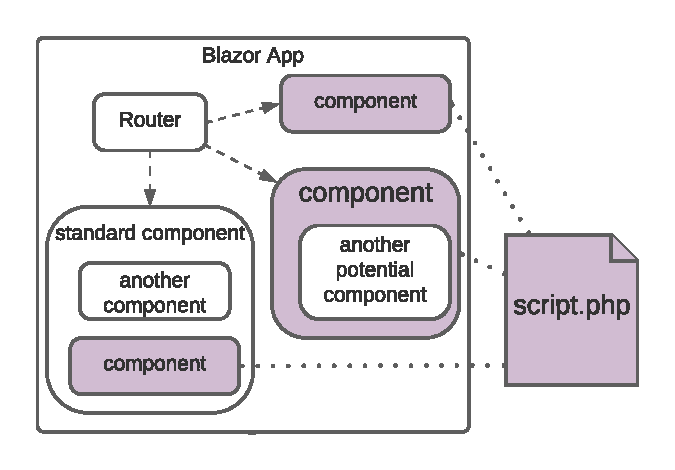
\includegraphics{./img/component}
\caption{The component representing a PHP script.}
\label{img02:component}
\end{figure} 
\par
We can think about how to represent PHP scripts as components.
There can be one type of component, which will provide the abstraction for all the PHP code in scenarios.
A problem with this approach is that the scenarios claim different levels of abstraction.
The third scenario wants to use the component for offering the Blazor interface accessible from PHP code.
The offer should contain identical or similar options, which are given in a C\# code.
The second scenario wants to use the component as an adjustable provider.
The provider finds and executes PHP scripts.
Its purpose is to keep the user away from knowing about the detailed structure of Blazor and the integration.
Another important thing is a provider's role in a Blazor App.
The provider can behave either as the Router or as a navigatable component, which enables the navigation of PHP scripts.
The conflict yields to create more types of components.
These types will provide the abstraction for the particular scenario.
The solution will reach two types of components.
The first one wants to bring Blazor to PHP in order to utilize the whole environment.
The second one aims to present transparent executing of standard PHP script without strangeness of connection between Blazor and PHP.
\par
We will focus on the first component.
We will call the component PhpComponent due to the effort of moving the component concept to PHP.
PhpComponent aims to the third scenario.
Despite language's differences, we can utilize the common concept of classes and inheritance.
Peachpie allows inheriting C\# class in a PHP code.
This feature results in full support of component interface without creating new structures for managing component's behavior from PHP.
We can inherit ComponentBase class in PHP and use its methods in the same way as C\# class.
The inheritance offers the required interface for creating effective rendering in scenario 3.
There are also subproblems with the differences.
The current Peachpie version does not support some C\# specifics fully.
The reason can be a hard or impossible representation of C\# entities in PHP.
It should be developed some PHP support for making the usage of the interface easier.
The support will replace the missing usage of the interface.
\par
We will call the second type of component by PhpScriptProvider expressing an environment for executing standard PHP scripts.
PhpScriptProvider aggregates the requirements of the rest scenarios by a single component.
Although, the provider has more than one purpose.
The main idea of serving a PHP code is the same.
The provider should be able to navigate and execute PHP scripts.
Because the rest scenarios try to hide the integration, the provider should support the following features.
It should pretend a server's behavior.
The behavior contains rendering everything, which is outside the PHP section or written by echo.
Superglobals are often used for obtaining additional information given by the user.
An ability to fill \$\_GET variable with the URL's query part should be presented.
It should change a standard Form functionality to saving the Form's information into superglobals and execute the script again.
Loading and saving files submitted by Form is essential for avoiding using Javascript.
There is an interesting thing about saving the script's context to the next execution.
These abilities are the same for the rest scenarios.
We will describe the provider's modes.
These modes are intended to solve the rest scenarios. 
\par
The first mode relates to the first scenario.
It enables to set the provider as a root component.
It handles all navigation events, determines the script's name, finds it, and executes the script.
PhpComponents can also be a navigation's target.
\par
The second mode relates to the second scenario.
It enables the provider's insertion into a Razor page.
Afterward, the provider executes the specified script.
\par
The third mode relates to the last scenario.
It enables to navigate the set of scripts with respect to URL.
The navigation is generally maintained by the default Router.
The component only provides navigation to scripts.
\par
We can see that two different components are rational ways how to separate the problems and offer an understandable difference between the components.


